% Options for packages loaded elsewhere
\PassOptionsToPackage{unicode}{hyperref}
\PassOptionsToPackage{hyphens}{url}
%
\documentclass[
  ignorenonframetext,
  aspectratio=169]{beamer}
\usepackage{pgfpages}
\setbeamertemplate{caption}[numbered]
\setbeamertemplate{caption label separator}{: }
\setbeamercolor{caption name}{fg=normal text.fg}
\beamertemplatenavigationsymbolsempty
% Prevent slide breaks in the middle of a paragraph
\widowpenalties 1 10000
\raggedbottom
\setbeamertemplate{part page}{
  \centering
  \begin{beamercolorbox}[sep=16pt,center]{part title}
    \usebeamerfont{part title}\insertpart\par
  \end{beamercolorbox}
}
\setbeamertemplate{section page}{
  \centering
  \begin{beamercolorbox}[sep=12pt,center]{part title}
    \usebeamerfont{section title}\insertsection\par
  \end{beamercolorbox}
}
\setbeamertemplate{subsection page}{
  \centering
  \begin{beamercolorbox}[sep=8pt,center]{part title}
    \usebeamerfont{subsection title}\insertsubsection\par
  \end{beamercolorbox}
}
\AtBeginPart{
  \frame{\partpage}
}
\AtBeginSection{
  \ifbibliography
  \else
    \frame{\sectionpage}
  \fi
}
\AtBeginSubsection{
  \frame{\subsectionpage}
}
\usepackage{amsmath,amssymb}
\usepackage{lmodern}
\usepackage{iftex}
\ifPDFTeX
  \usepackage[T1]{fontenc}
  \usepackage[utf8]{inputenc}
  \usepackage{textcomp} % provide euro and other symbols
\else % if luatex or xetex
  \usepackage{unicode-math}
  \defaultfontfeatures{Scale=MatchLowercase}
  \defaultfontfeatures[\rmfamily]{Ligatures=TeX,Scale=1}
\fi
\usetheme[]{Frankfurt}
\usecolortheme{beaver}
% Use upquote if available, for straight quotes in verbatim environments
\IfFileExists{upquote.sty}{\usepackage{upquote}}{}
\IfFileExists{microtype.sty}{% use microtype if available
  \usepackage[]{microtype}
  \UseMicrotypeSet[protrusion]{basicmath} % disable protrusion for tt fonts
}{}
\makeatletter
\@ifundefined{KOMAClassName}{% if non-KOMA class
  \IfFileExists{parskip.sty}{%
    \usepackage{parskip}
  }{% else
    \setlength{\parindent}{0pt}
    \setlength{\parskip}{6pt plus 2pt minus 1pt}}
}{% if KOMA class
  \KOMAoptions{parskip=half}}
\makeatother
\usepackage{xcolor}
\newif\ifbibliography
\setlength{\emergencystretch}{3em} % prevent overfull lines
\providecommand{\tightlist}{%
  \setlength{\itemsep}{0pt}\setlength{\parskip}{0pt}}
\setcounter{secnumdepth}{-\maxdimen} % remove section numbering
\usepackage{booktabs}
\usepackage{longtable}
\usepackage{array}
\usepackage{multirow}
\usepackage{wrapfig}
\usepackage{float}
\usepackage{colortbl}
\usepackage{pdflscape}
\usepackage{tabu}
\usepackage{threeparttable}
\usepackage{threeparttablex}
\usepackage[normalem]{ulem}
\usepackage{makecell}
\usepackage{xcolor}
\usepackage{tikz} % required for image opacity change
\usepackage[absolute,overlay]{textpos} % for text formatting

% this font option is amenable for beamer
\setbeamerfont{caption}{size=\tiny}

\newcommand{\bcolumns}{\begin{columns}[T, onlytextwidth]}
\newcommand{\ecolumns}{\end{columns}}

\newcommand{\bdescription}{\begin{description}}
\newcommand{\edescription}{\end{description}}

\newcommand{\bitemize}{\begin{itemize}}
\newcommand{\eitemize}{\end{itemize}}
\AtBeginSubsection{}
\ifLuaTeX
  \usepackage{selnolig}  % disable illegal ligatures
\fi
\usepackage[]{natbib}
\bibliographystyle{plainnat}
\IfFileExists{bookmark.sty}{\usepackage{bookmark}}{\usepackage{hyperref}}
\IfFileExists{xurl.sty}{\usepackage{xurl}}{} % add URL line breaks if available
\urlstyle{same} % disable monospaced font for URLs
\hypersetup{
  pdftitle={Genetic diversity and center of diversity of crops},
  hidelinks,
  pdfcreator={LaTeX via pandoc}}

\title{Genetic diversity and center of diversity of crops}
\author{Deependra Dhakal\\
Assistant Professor\\
Agriculture and Forestry University\\
\textit{ddhakal.rookie@gmail.com}\\
\url{https://rookie.rbind.io}}
\date{}

\begin{document}
\frame{\titlepage}

\begin{frame}[allowframebreaks]
  \tableofcontents[hideallsubsections]
\end{frame}
\hypertarget{species-and-genetic-diversity}{%
\section{Species and genetic
diversity}\label{species-and-genetic-diversity}}

\begin{frame}{Genetic diversity}
\protect\hypertarget{genetic-diversity}{}
\begin{itemize}
\tightlist
\item
  Is reliant on the heritable variation within and between populations
  of organisms.
\item
  Genetic variation (new) arises by gene and chromosome mutations, and
  through recombination.
\item
  It has been estimated that in humans and fruit flies alike, the number
  of possible combinations of different forms of each gene sequence
  exceeds the number of atoms in the universe.
\item
  Genetic variation enables both natural evolutionary change and
  artificial selective breeding to occur.
\item
  Only a small fraction (\textless1\%) of the genetic material of higher
  organisms is outwardly expressed in the form and function of the
  organism; the purpose of the remaining DNA and the significance of any
  variation within it are unclear.
\end{itemize}
\end{frame}

\begin{frame}{}
\protect\hypertarget{section}{}
\begin{itemize}
\item
  Before initiating a (molecular/marker-assisted) breeding program an
  assessment of genetic diversity of the available germplasm is
  necessary.
\item
  The goal is to select parents that are genetically diverse enough that
  you can identify differences - polymorphisms - in the progeny.
\item
  Of several, few of the measures of genetic diversity are:

  \begin{itemize}
  \footnotesize
  \item Based on the number of variants among the alleles
  \item Polymorphism or rate of polymorphism (Pj)
  \item Proportion of polymorphic loci
  \item Number of alleles (A) and allelic richness (As)
  \item Average number of alleles per locus
  \item Based on the frequency of variant alleles
  \item Average expected heterozygosity (He; Nei’s genetic diversity)
  \end{itemize}
\item
  Clearly the use of markers is needed for these measures of genetic
  diversity.
\item
  The genetic distance between two samples is described as the
  proportion of genetic elements (alleles, genes, gametes, genotypes)
  that the two samples do not share.
\end{itemize}
\end{frame}

\begin{frame}{}
\protect\hypertarget{section-1}{}
\scriptsize

A study of 26 accessions of groundnut (consisting of interspecific
derivatives, land races and released cultivars) and 8 primers of a
10-mer were selected for RAPD DNA assay. The genetic similarity
(\(S_{ij}\)) ranged from 59.0\% to 98.8\%, with an average of 86.2\%.
Both multidimensional scaling and unweighted pair-group method with
arithmetic averages (UPGMA) dendrograms revealed the existence of five
distinct clusters. However, this classification could not be related to
known biological information about the accessions falling into di?erent
clusters. Some accessions with diverse DNA profiles (ICG 1448, 7101, and
1471, and ICGV 99006 and 99014) were identified for mapping and genetic
enhancement in groundnut. \citep{dwivedi2001assessment}.

\begin{center}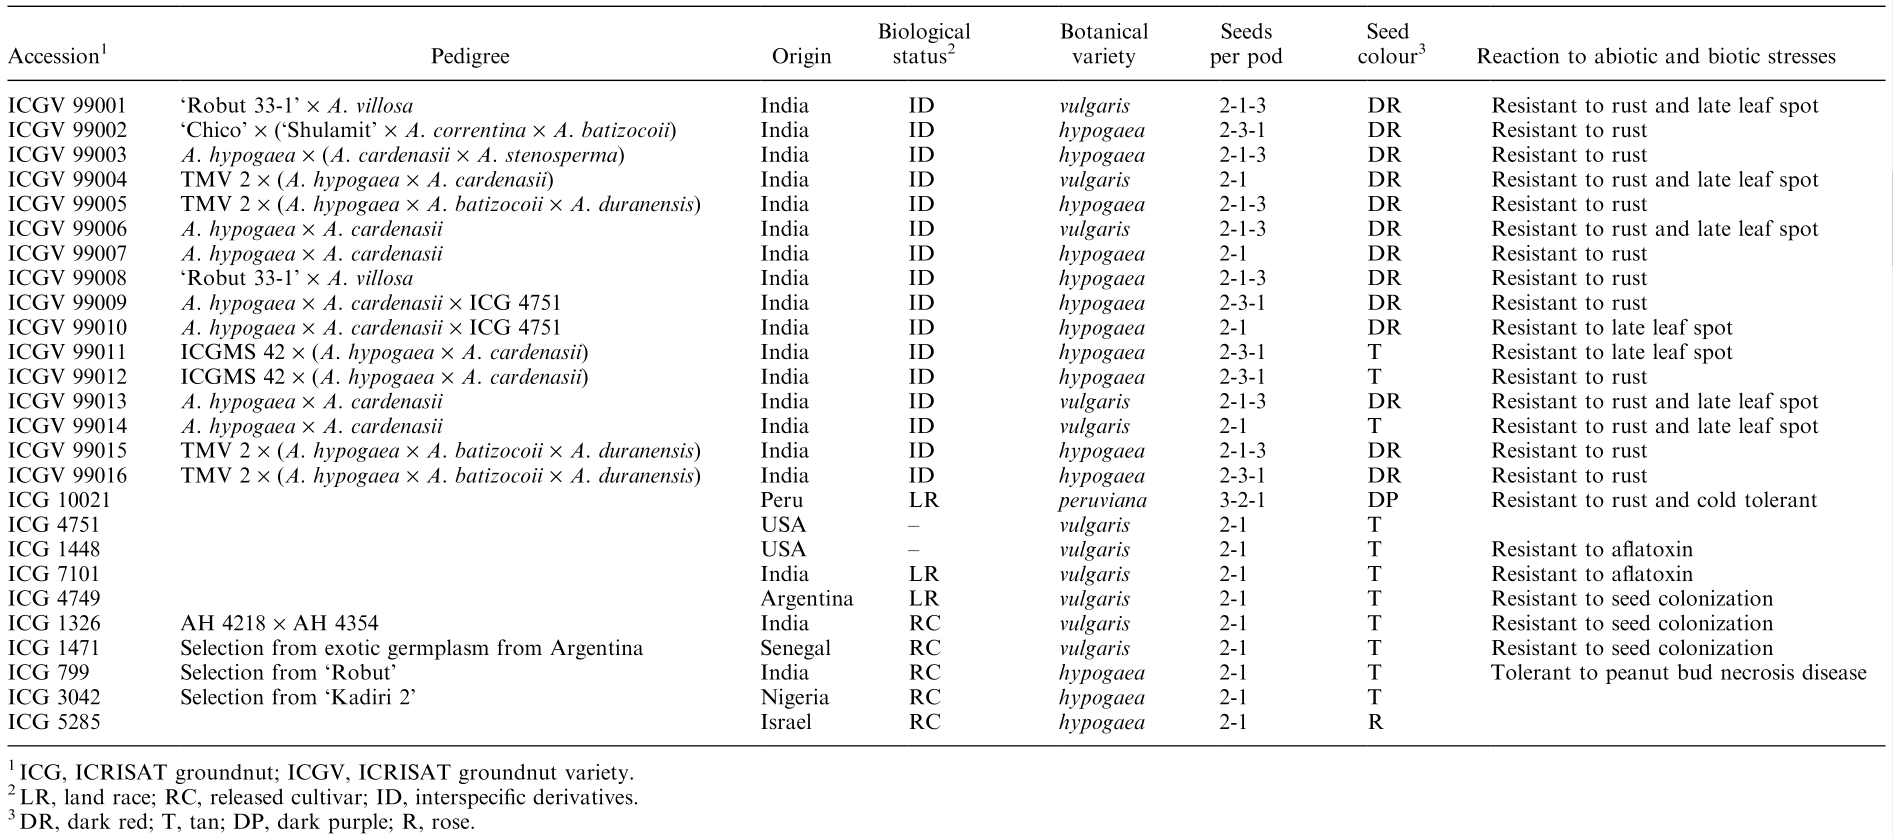
\includegraphics[width=0.8\linewidth]{../images/Groundnut_diversity} \end{center}
\end{frame}

\begin{frame}{}
\protect\hypertarget{section-2}{}
\bcolumns
\column{0.5\textwidth}
\scriptsize

A study conducted in \textbf{Ghana} evaluated 142 soybean accessions,
genotyped with 34 SSR markers. 5 quantitative and 2 qualitative traits
were concurrently evaluated. 29 of the SSR markers were polymorphic with
mean allele number of 5.3, PIC of 0.51 and gene diversity of 0.55. UPGMA
clustering and Principal Coordinate Analysis was similar in explaining
the extent of diversity within the accessions. Structure analysis placed
most of the accessions into two subpopulations with 18 (12.7\%) as
admixtures. Both UPGMA clustering-based SSR data and PCA from phenotypic
data showed similar results\citep{denwar2019genetic}.

\column{0.5\textwidth}

\begin{center}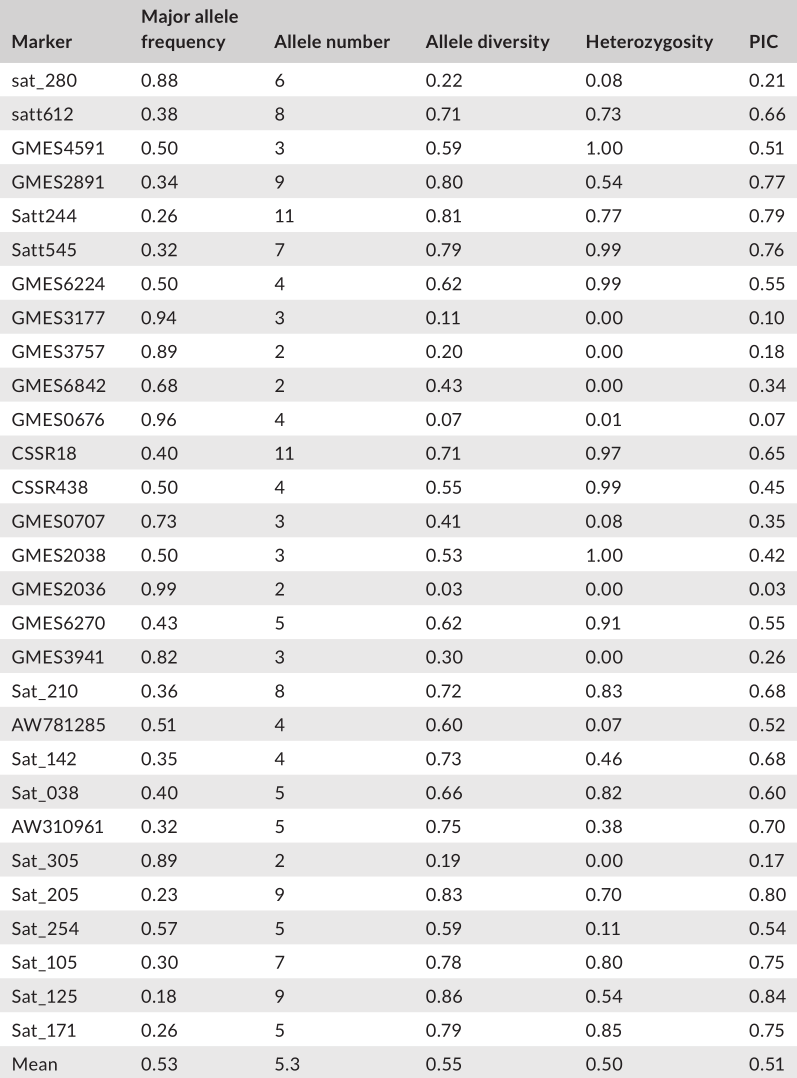
\includegraphics[width=0.8\linewidth]{../images/Ghana_soybean_diversity} \end{center}

\ecolumns
\end{frame}

\begin{frame}{}
\protect\hypertarget{section-3}{}
\begin{center}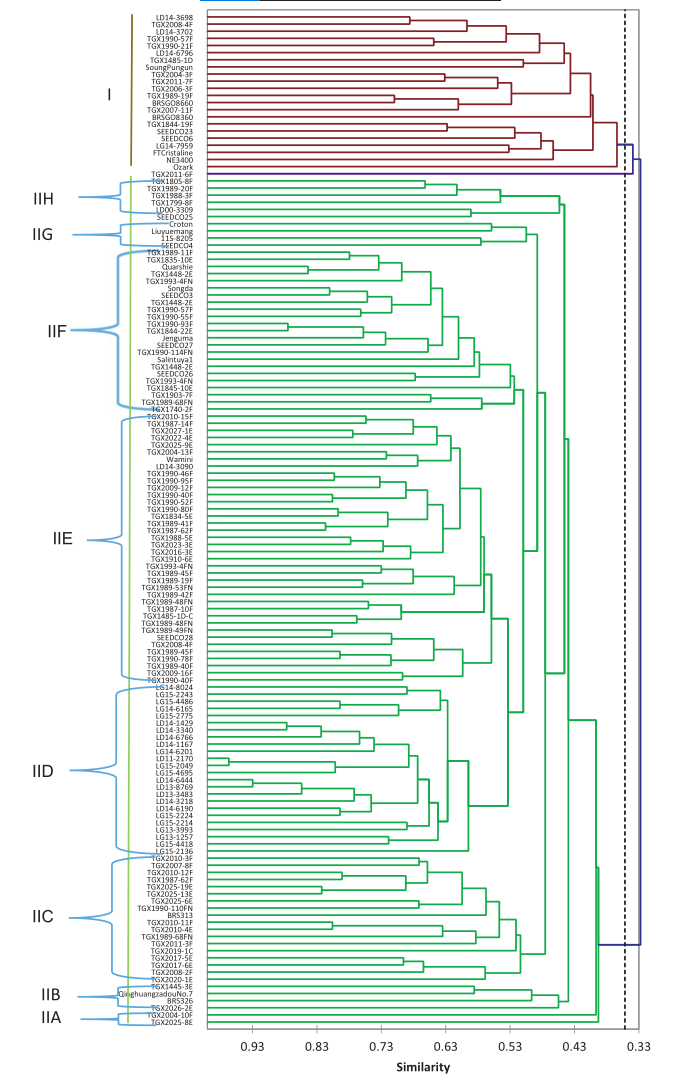
\includegraphics[width=0.4\linewidth]{../images/Ghana_soybean_upgma_clustering} \end{center}
\end{frame}

\begin{frame}{}
\protect\hypertarget{section-4}{}
\begin{center}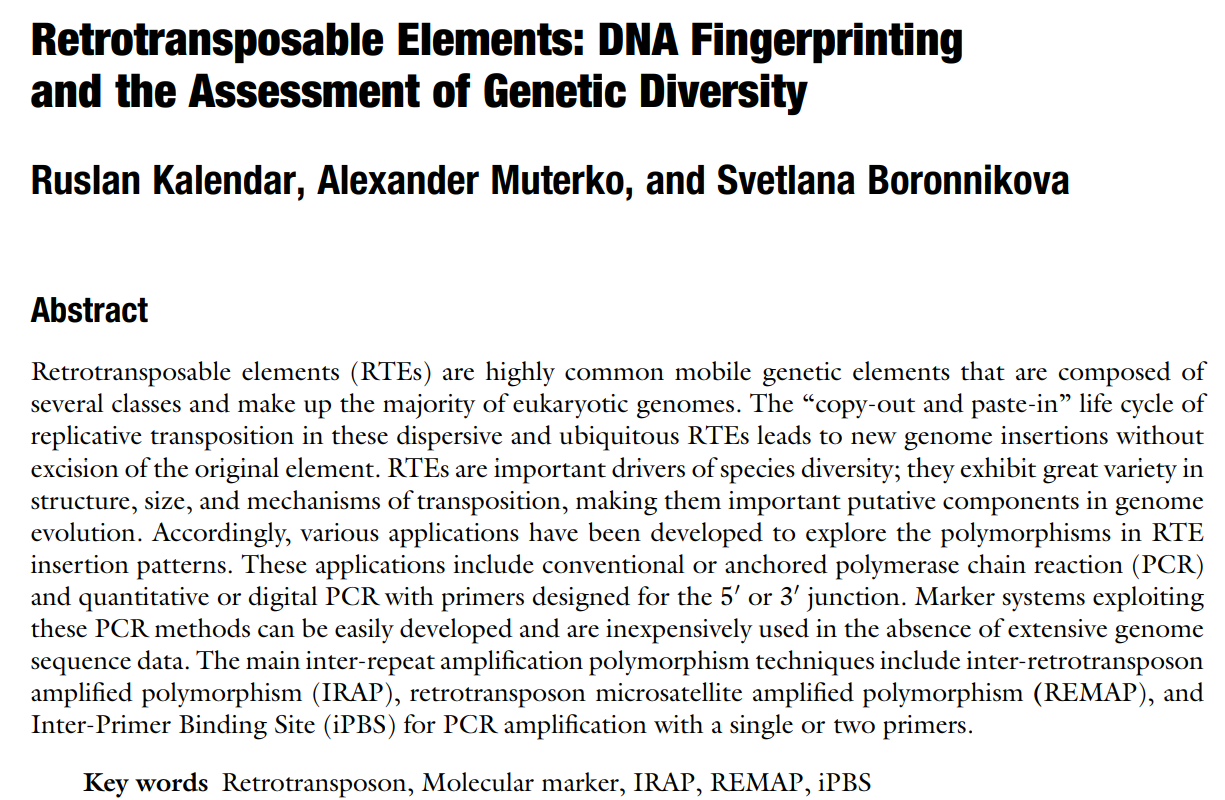
\includegraphics[width=0.76\linewidth]{../images/Transposon_fingerprinting_genetic_diversity_assess} \end{center}

For the extensive discussion and protocol outline, refer to
\citet{kalendar2021retrotransposable}.
\end{frame}

\begin{frame}{}
\protect\hypertarget{section-5}{}
\begin{center}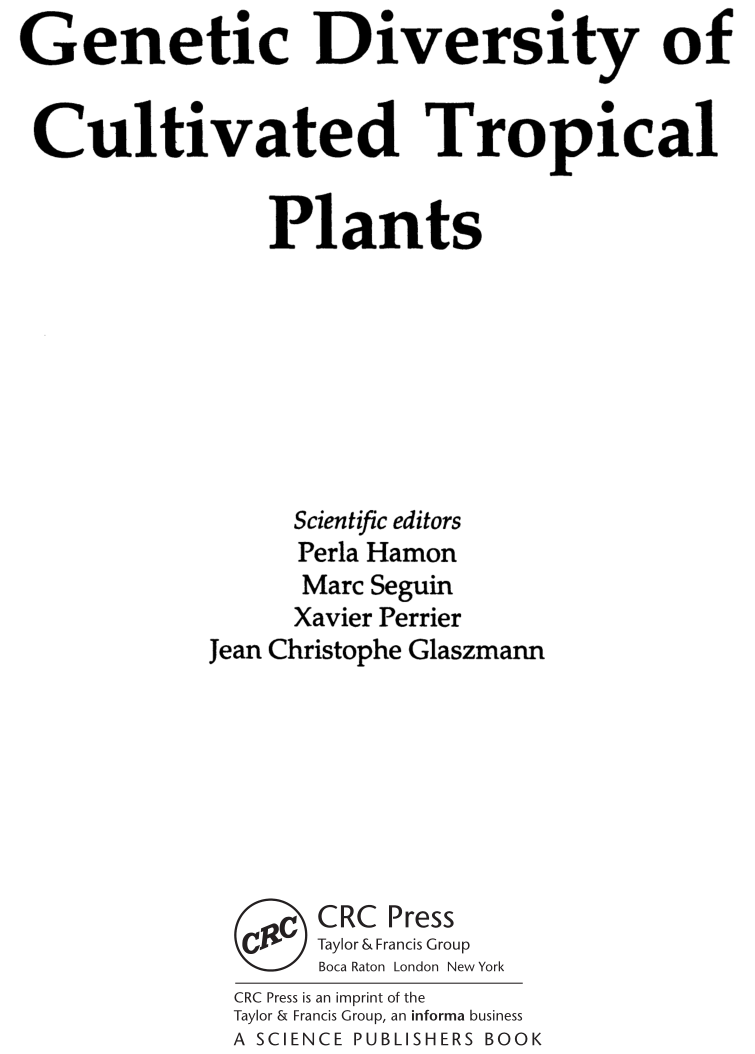
\includegraphics[width=0.5\linewidth]{../images/Genetic_diversity_of_cultivated_plants_textbook} \end{center}
\end{frame}

\begin{frame}{Species diversity}
\protect\hypertarget{species-diversity}{}
\begin{itemize}
\tightlist
\item
  Species are the fundamental descriptive units of the living world and
  this is why biodiversity is very commonly, and \textbf{incorrectly},
  used as a synonym of species diversity, in particular of ``species
  richness''.
\item
  When considering species numbers alone, life on earth appears to
  consist mostly of insects and microorganisms.
\item
  The greater the interspecific differences (e.g., by an isolated
  position within the taxonomic hierarchy), then the greater
  contribution to any overall measure of global biological diversity --
  implicit by the term ``biodiversity''.
\item
  The ecological importance of a species can have a direct effect on
  community structure, and thus on overall biological diversity. For
  example, a species of tropical rain forest tree that supports an
  endemic invertebrate fauna of a hundred species makes a greater
  contribution to the maintenance of global biological diversity than
  does a European alpine plant that may have no other species wholly
  dependent on it.
\item
  In a seminal work on the measurement of diversity, Whittaker (1972)
  introduced the concepts of alpha, beta, and gamma diversity. The
  measurements with Shannon Weaner formula, giving diversity values for
  single sites, are examples of alpha diversity.
\item
  For a history of approaches to measurement and defining of species
  diversity, refer to Page 476 of Encyclopedia of Biodiversity.
\end{itemize}

(Refer to Page 206 of Encyclopedia of Biodiversity for example and
illustrations on Agrobiodiversity.)

\begin{center}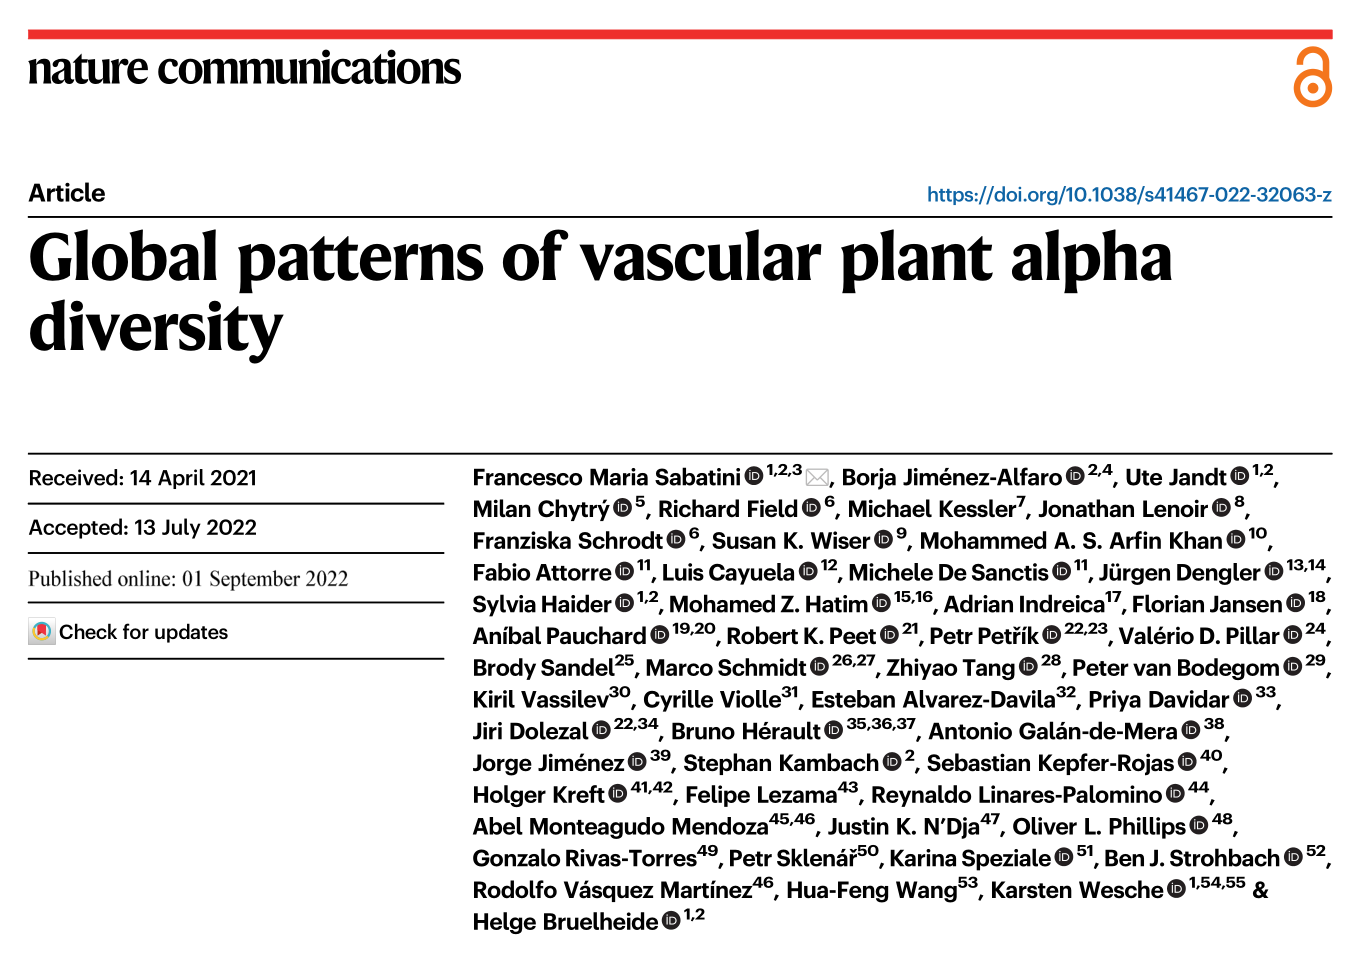
\includegraphics[width=0.6\linewidth]{../images/global_pattern_alpha_diversity} \end{center}
\end{frame}

\begin{frame}{Germplasm}
\protect\hypertarget{germplasm}{}
\begin{itemize}
\tightlist
\item
  Germplasm refers to the genetic material that can be used to
  perpetuate a species or population
\item
  Germplasm provides the material used to initiate a breeding program
\item
  Sometimes only germplasm screening and evaluation is practiced for
  introduction of improved variety in a region
\item
  Certain institutional sets-ups such as gene banks are charged with the
  responsibility of assembling, cataloguing, storing and managing large
  number of germplasm. This allows for quick retrieval.
\end{itemize}
\end{frame}

\begin{frame}{Gene pool}
\protect\hypertarget{gene-pool}{}
J.R. Harlan and J.M.J. de Wet proposed a categorization of gene pools of
cultivated crops according to the feasibility of gene transfer or gene
flow from those species to the crop species.

\bcolumns
\column{0.65\textwidth}

\begin{figure}
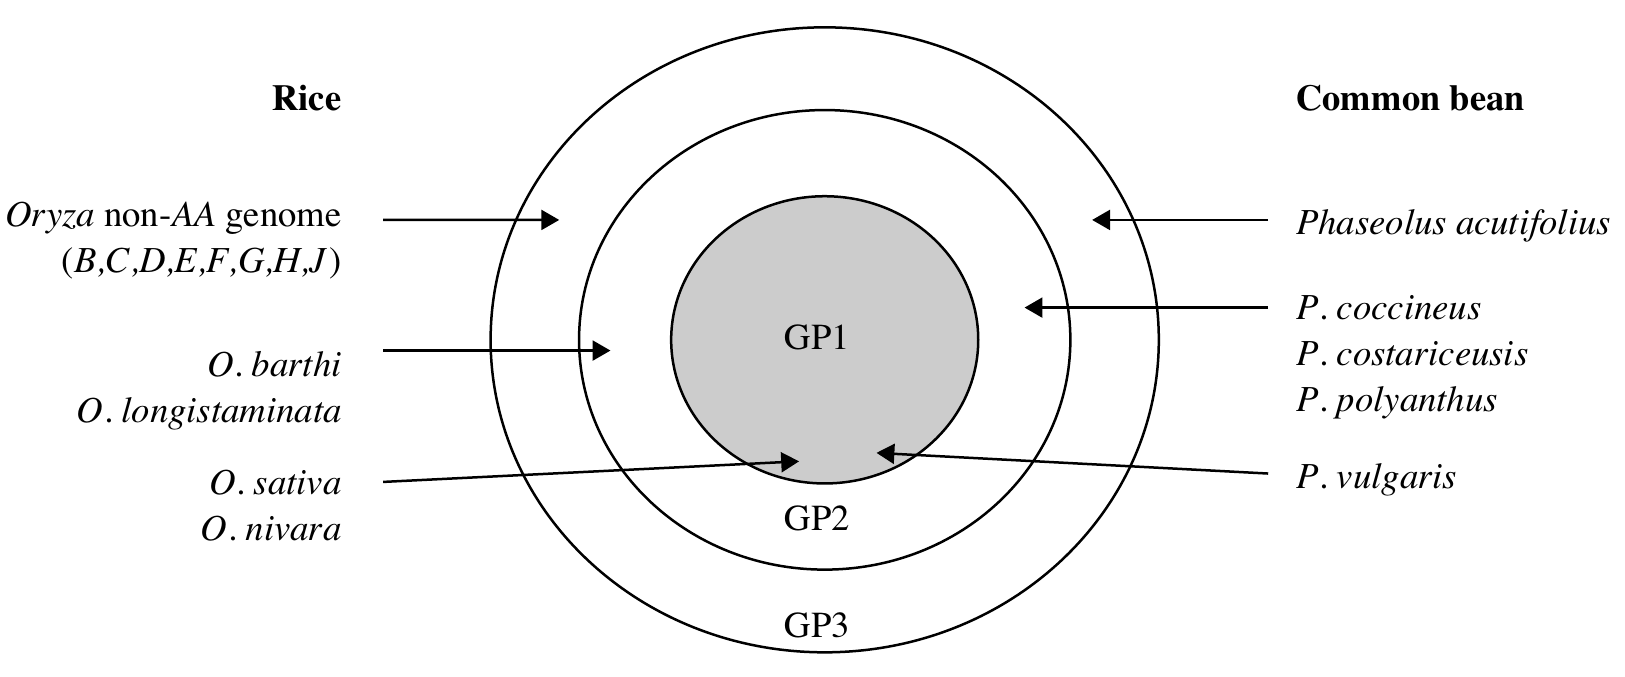
\includegraphics[width=0.9\linewidth]{../images/crop_gene_pools} \caption{Crop gene pools; A system proposed by Harlan}\label{fig:gene-pools}
\end{figure}

\column{0.35\textwidth}

\begin{figure}
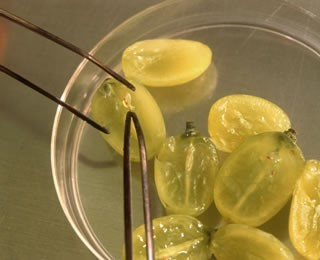
\includegraphics[width=0.98\linewidth]{../images/embryo_rescue} \caption{The embryo rescue of grape seeds. Increasing diversity by introgression from wild relatives can be complicated by the existence of crossing barriers or poor hybrid fertility.}\label{fig:embryo-resuce}
\end{figure}

\ecolumns
\end{frame}

\begin{frame}{Types of gene pool}
\protect\hypertarget{types-of-gene-pool}{}
\small

\begin{itemize}
\tightlist
\item
  \emph{Primary gene pool (GP1)}

  \begin{itemize}
  \tightlist
  \item
    GP1 consists of biological species that can be intercrossed easily
    (interfertile) without any problems with fertility of the progeny.
    That is, there is no restriction to gene exchange between members of
    the group. This group may contain both cultivated and wild
    progenitors of the species.
  \end{itemize}
\item
  \emph{Secondary gene pool (GP2)}

  \begin{itemize}
  \tightlist
  \item
    Members of this gene pool include both cultivated and wild relatives
    of the crop species. They are more distantly related and have
    crossability problems. Nonetheless, crossing produces hybrids and
    derivatives that are sufficiently fertile to allow gene flow. GP2
    species can cross with those in GP1, with some fertility of the F1,
    but more difficulty with success.
  \end{itemize}
\item
  \emph{Tertiary gene pool (GP3)}

  \begin{itemize}
  \tightlist
  \item
    GP3 involves the outer limits of potential genetic resources. Gene
    transfer by hybridization between GP1 and GP3 is very problematic,
    resulting in lethality, sterility, and other abnormalities. To
    exploit germplasm from distant relatives, tools such as embryo
    rescue and bridge crossing may be used to nurture an embryo from a
    wide cross to a full plant and to obtain fertile plants.
  \end{itemize}
\end{itemize}
\end{frame}

\hypertarget{wild-genetic-diversity-of-some-important-crops}{%
\section{Wild genetic diversity of some important
crops}\label{wild-genetic-diversity-of-some-important-crops}}

\begin{frame}{Domestication}
\protect\hypertarget{domestication}{}
\begin{block}{}
a plant population has been domesticated when it has been substantially altered from the wild state and certainly when it has been so altered to be unable to survive in the wild
\end{block}

N.W. Simmonds

\begin{itemize}
\tightlist
\item
  Domestication is the process by which genetic changes (shifts) in wild
  plants are brought about through a selection process imposed by
  humans.
\end{itemize}
\end{frame}

\hypertarget{domestication-syndrome-changes-in-plant-species-under-domestication}{%
\subsection{Domestication syndrome (Changes in plant species under
domestication)}\label{domestication-syndrome-changes-in-plant-species-under-domestication}}

\begin{frame}{Domestication syndrome (Changes in plant species under
domestication)}
\begin{table}

\caption{\label{tab:domestication-syndrome}Changes in plants under domestication}
\centering
\fontsize{6}{8}\selectfont
\begin{tabular}[t]{>{\raggedright\arraybackslash}p{16em}>{\raggedright\arraybackslash}p{40em}}
\toprule
General effect & Specific traits altered\\
\midrule
\textbf{\cellcolor{gray!6}{Increased seedling vigor (more plants germinating)}} & \cellcolor{gray!6}{Loss of seed or tuber dormancy}\\
\textbf{} & Large seeds\\
\textbf{\cellcolor{gray!6}{Modified reproductive system}} & \cellcolor{gray!6}{Increased selfing}\\
\textbf{} & Reduced complexity of reproductive organs\\
\textbf{\cellcolor{gray!6}{}} & \cellcolor{gray!6}{Vegetatively reproducing plants}\\
\addlinespace
\textbf{} & Altered photoperiod sensitivity\\
\textbf{\cellcolor{gray!6}{}} & \cellcolor{gray!6}{Shift in sex form of species}\\
\textbf{} & Promotion of asexual reproduction\\
\textbf{\cellcolor{gray!6}{Increased number of seeds harvested}} & \cellcolor{gray!6}{Non-shattering}\\
\textbf{} & Reduced number of branches (more fruits per branch)\\
\bottomrule
\end{tabular}
\end{table}
\end{frame}

\begin{frame}{}
\protect\hypertarget{section-6}{}
\begin{table}

\caption{\label{tab:domestication-syndrome2}Changes in plants under domestication\footnote[frame]{For a detailed contrast between wild and domestication traits, refer to Lecture on 'Domestication, plant introduction, and acclimatization' of Introductory Plant Breeding course.} (...continued)}
\centering
\fontsize{6}{8}\selectfont
\begin{tabular}[t]{>{\raggedright\arraybackslash}p{16em}>{\raggedright\arraybackslash}p{40em}}
\toprule
General effect & Specific traits altered\\
\midrule
\textbf{\cellcolor{gray!6}{Increased appeal to consumers}} & \cellcolor{gray!6}{Attractive fruit/seed colors and patterns}\\
\textbf{} & Enhanced flavor, texture, and taste of seeds/fruits/tubers (food parts)\\
\textbf{\cellcolor{gray!6}{}} & \cellcolor{gray!6}{Reduced toxic principles (safer food)}\\
\textbf{} & Larger fruits\\
\textbf{\cellcolor{gray!6}{}} & \cellcolor{gray!6}{Reduces spikiness}\\
\addlinespace
\textbf{} & Increase in economic yield (HI)\\
\textbf{\cellcolor{gray!6}{Altered plant architecture and growth habit}} & \cellcolor{gray!6}{Compact growth habit (Determinacy, reduced plant size, dwarfism)}\\
\textbf{} & Reduced branching\\
\textbf{\cellcolor{gray!6}{}} & \cellcolor{gray!6}{Decreases in variability within a variety}\\
\textbf{Change in developmental phenology} & Change in life cycle (normally from perennial to annual for seed crops, and from annual to biennial for vegetable crops)\\
\bottomrule
\end{tabular}
\end{table}
\end{frame}

\hypertarget{origin-and-diversity}{%
\section{Origin and diversity}\label{origin-and-diversity}}

\begin{frame}{Law of homologous series of variation}
\protect\hypertarget{law-of-homologous-series-of-variation}{}
\begin{itemize}
\tightlist
\item
  Nikolai I. Vavilov (1887-1942), the Russian botanist and plant
  breeder, demonstrated the existence of `centres of origin' of
  cultivated plants (more correctly named today as `centres of
  diversity'), in which can be found the highest level of genetic
  variability of a species. This variability, which arises in nature by
  mutation spontaneous hybridization, introgression and changes in
  chromosome form and number, provides the means by which adaptation to
  heterogenous environments can occur.
\item
  It allows the breeder to identify sources of variation for specific
  characteristics. The extension of this principle to related species
  was formulated by Vavilov in his `law of homologous series of
  variation'. This law allows the prediction of the appearance of a
  given type of mutation in a plant species when such a type has been
  found in another species phylogenetically related to the first.
\item
  Defined plant breeding as `plant evolution directed by man'; concept
  of `applied plant genetics'.
\end{itemize}
\end{frame}

\begin{frame}{Defining center of origin and center of diversity}
\protect\hypertarget{defining-center-of-origin-and-center-of-diversity}{}
\begin{itemize}
\tightlist
\item
  CBD takes the ``centre of origin'' and the ``centre of crop
  diversity'' as references referring to the scientific rather than
  political connecting points for the definition of origin. {[}Rights to
  plant genetic resources and traditional knowledge{]}
\item
  It defines ``centre of origin'' as ``a geographical area where a plant
  species, either domesticated or wild, first developed its distinctive
  properties'', and ``centre of crop diversity'' as ``the geographic
  area containing a high level of genetic diversity for crop species in
  in-situ conditions'' (Articles 2.8 and 2.9).
\item
  On the basis of soveignty of states over their natural resources, CBD
  takes ``country'' as starting point for defining the origin of genetic
  resources.
\item
  Accordingly, ``the country of origin of genetic resources'' is defined
  as the country that possesses the genetic resources in in situ
  conditions (Article 2.4).
\end{itemize}
\end{frame}

\begin{frame}{Domestication and origin of major crop species}
\protect\hypertarget{domestication-and-origin-of-major-crop-species}{}
\begin{table}

\caption{\label{tab:domestication-origin}Estimated time of domestication and centre of origin of major crop species; \cite{brown2014plant}, Page 23.}
\centering
\fontsize{6}{8}\selectfont
\begin{tabular}[t]{>{\raggedright\arraybackslash}p{8em}>{\raggedright\arraybackslash}p{12em}>{\raggedright\arraybackslash}p{8em}>{\raggedright\arraybackslash}p{12em}}
\toprule
Crop category & Crop & Length of time domesticated (years) & Possible region of origin\\
\midrule
\textbf{\cellcolor{gray!6}{Cereals}} & \cellcolor{gray!6}{Maize, Zea mays} & \cellcolor{gray!6}{7000} & \cellcolor{gray!6}{Mexico, Central America}\\
\textbf{Cereals} & Rice, Oryza sativa & 4500 & Thailand, Southern China\\
\textbf{\cellcolor{gray!6}{Cereals}} & \cellcolor{gray!6}{Wheat, Triticum spp.} & \cellcolor{gray!6}{8500} & \cellcolor{gray!6}{Syria, Jordan, Israel, Iraq}\\
\textbf{Cereals} & Barley, Hordeum vulgare & 9000 & Syria, Jordan, Israel, Iraq\\
\textbf{\cellcolor{gray!6}{Cereals}} & \cellcolor{gray!6}{Sorghum, Sorghum bicolor} & \cellcolor{gray!6}{8000} & \cellcolor{gray!6}{Equatorial Africa}\\
\addlinespace
\textbf{Oilseeds} & Soybean, Glycine max & 2000 & North China\\
\textbf{\cellcolor{gray!6}{Oilseeds}} & \cellcolor{gray!6}{Oil palm, Elaeis guineensis} & \cellcolor{gray!6}{9000} & \cellcolor{gray!6}{Central Africa}\\
\textbf{Oilseeds} & Coconut palm, Cocos nucifera & 100 & Southern Asia\\
\textbf{\cellcolor{gray!6}{Oilseeds}} & \cellcolor{gray!6}{Rapeseed, Brassica napus} & \cellcolor{gray!6}{500} & \cellcolor{gray!6}{Mediterranean Europe}\\
\textbf{Oilseeds} & Sunflower, Helianthus annus & 3000 & Western United States\\
\addlinespace
\textbf{\cellcolor{gray!6}{Pulses}} & \cellcolor{gray!6}{Beans, Phaseolus spp} & \cellcolor{gray!6}{7000} & \cellcolor{gray!6}{Centra America, Mexico}\\
\textbf{Pulses} & Lentil, Lens culinaris & 7000 & Syria, Jordan, Israel, Iraq\\
\textbf{\cellcolor{gray!6}{Pulses}} & \cellcolor{gray!6}{Peas, Pisum sativum} & \cellcolor{gray!6}{9000} & \cellcolor{gray!6}{Syria, Jordan, Israel, Iraq}\\
\textbf{Root crops} & Potato, Solanum tuberosum & 7000 & Peru\\
\textbf{\cellcolor{gray!6}{Root crops}} & \cellcolor{gray!6}{Cassava, Manihot esculenta} & \cellcolor{gray!6}{5000} & \cellcolor{gray!6}{Brazil, Mexico}\\
\bottomrule
\end{tabular}
\end{table}
\end{frame}

\begin{frame}{}
\protect\hypertarget{section-7}{}
\begin{table}

\caption{\label{tab:domestication-origin2}Estimated time of domestication and centre of origin of major crop species; \cite{brown2014plant}, Page 23 (...continued).}
\centering
\fontsize{6}{8}\selectfont
\begin{tabular}[t]{>{\raggedright\arraybackslash}p{8em}>{\raggedright\arraybackslash}p{12em}>{\raggedright\arraybackslash}p{8em}>{\raggedright\arraybackslash}p{12em}}
\toprule
Crop category & Crop & Length of time domesticated (years) & Possible region of origin\\
\midrule
\textbf{\cellcolor{gray!6}{Root crops}} & \cellcolor{gray!6}{Sweet potato, Ipomoea batatas} & \cellcolor{gray!6}{6000} & \cellcolor{gray!6}{South Central America}\\
\textbf{Root crops} & Sugar beet, Beta vulgaris & 300 & Mediterranean Europe\\
\textbf{\cellcolor{gray!6}{Vegetables}} & \cellcolor{gray!6}{Tomato, Lycopersicum esculentum} & \cellcolor{gray!6}{3000} & \cellcolor{gray!6}{Western South America}\\
\textbf{Vegetables} & Cabbage, Brassica oleracea & 3000 & Mediterranean Europe\\
\textbf{\cellcolor{gray!6}{Vegetables}} & \cellcolor{gray!6}{Onion, Allium spp.} & \cellcolor{gray!6}{4500} & \cellcolor{gray!6}{Iran, Afganistan, Pakistan}\\
\addlinespace
\textbf{Fruit} & Orange, Citrus sinensis & 9000 & South-east Asia\\
\textbf{\cellcolor{gray!6}{Fruit}} & \cellcolor{gray!6}{Apple, Malus spp.} & \cellcolor{gray!6}{3000} & \cellcolor{gray!6}{Asia Minor, Central Asia}\\
\textbf{Fruit} & Grape, Vitis spp. & 7000 & Eastern Asia\\
\textbf{\cellcolor{gray!6}{Fruit}} & \cellcolor{gray!6}{Banana, Musa acuminata, M. balbisiana} & \cellcolor{gray!6}{4500} & \cellcolor{gray!6}{South-east Asia}\\
\textbf{Others} & Cotton, Gossypium spp. & 4500 & Centra America, Brazil\\
\addlinespace
\textbf{\cellcolor{gray!6}{Others}} & \cellcolor{gray!6}{Coffee, Coffea spp.} & \cellcolor{gray!6}{500} & \cellcolor{gray!6}{West Ethiopia}\\
\textbf{Others} & Rubber, Hevea brasiliensis & 200 & Brazil, Bolivia, Paraguay\\
\textbf{\cellcolor{gray!6}{Others}} & \cellcolor{gray!6}{Alfalfa, Medicago sativa} & \cellcolor{gray!6}{4000} & \cellcolor{gray!6}{Iran, Northern Pakistan}\\
\bottomrule
\end{tabular}
\end{table}
\end{frame}

\begin{frame}{Rice: History and origin}
\protect\hypertarget{rice-history-and-origin}{}
\begin{itemize}
\tightlist
\item
  Probably originated 130 MYA (Virmani and IIyas-Ahmed, 2007)
\item
  Spread as wild grass in Gondwanaland.
\item
  Domesticated independently in Asia and Africa.

  \begin{itemize}
  \tightlist
  \item
    \emph{O. sativa} (derived from \emph{O. rufipogon} in China and in
    India)

    \begin{itemize}
    \tightlist
    \item
      Asian wild progenitor called \emph{O. rufipogon} has also
      perennial to annual types
    \item
      Annual types of the wild progenitor called \emph{O. nivara}
      resulted in present day asian rice
    \end{itemize}
  \item
    \emph{O. glaberrima} (derived from \emph{O. barthii} in the Niger
    river delta)
  \end{itemize}
\item
  Both cultivated species -- \emph{O. sativa} and \emph{O. glaberrima}
  (tropical West african rice) originated from common ancestor.
\item
  Alternative hypotheses: two distinct subspecies of rice (
  \emph{indica} and \emph{japonica}) arose from different wild variants
  of \emph{O. rufipogon}.
\end{itemize}
\end{frame}

\begin{frame}{}
\protect\hypertarget{section-8}{}
\bcolumns
\column{0.5\textwidth}

\begin{figure}
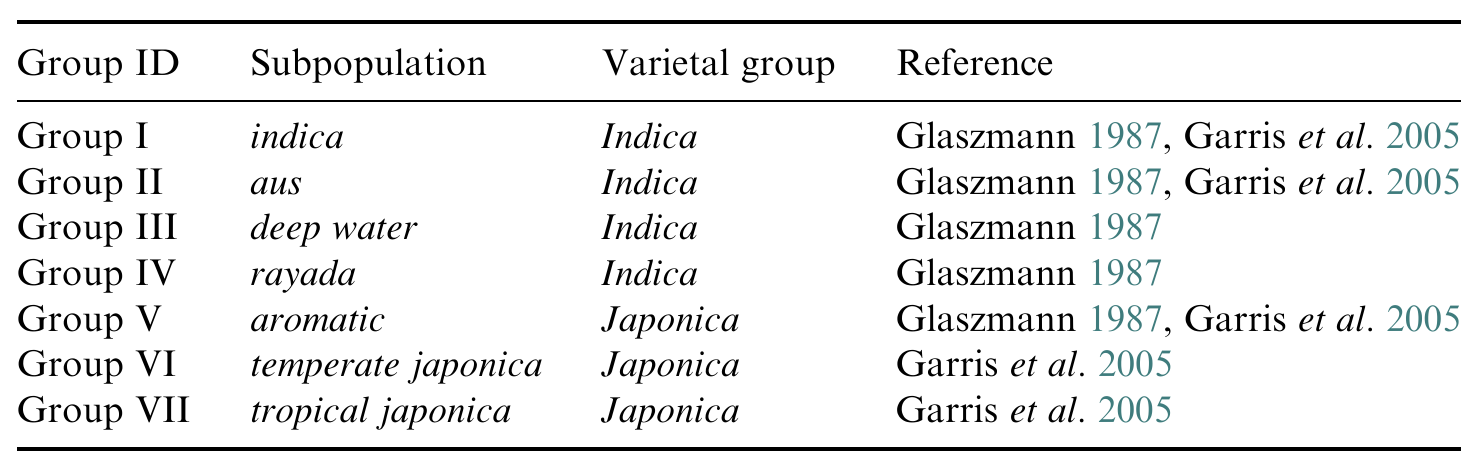
\includegraphics[width=0.94\linewidth]{./../images/rice_subpopulations} \caption{The recognized subpopulations of \textit{Oryza sativa}}\label{fig:subpopulations-rice}
\end{figure}

\column{0.5\textwidth}

\begin{figure}
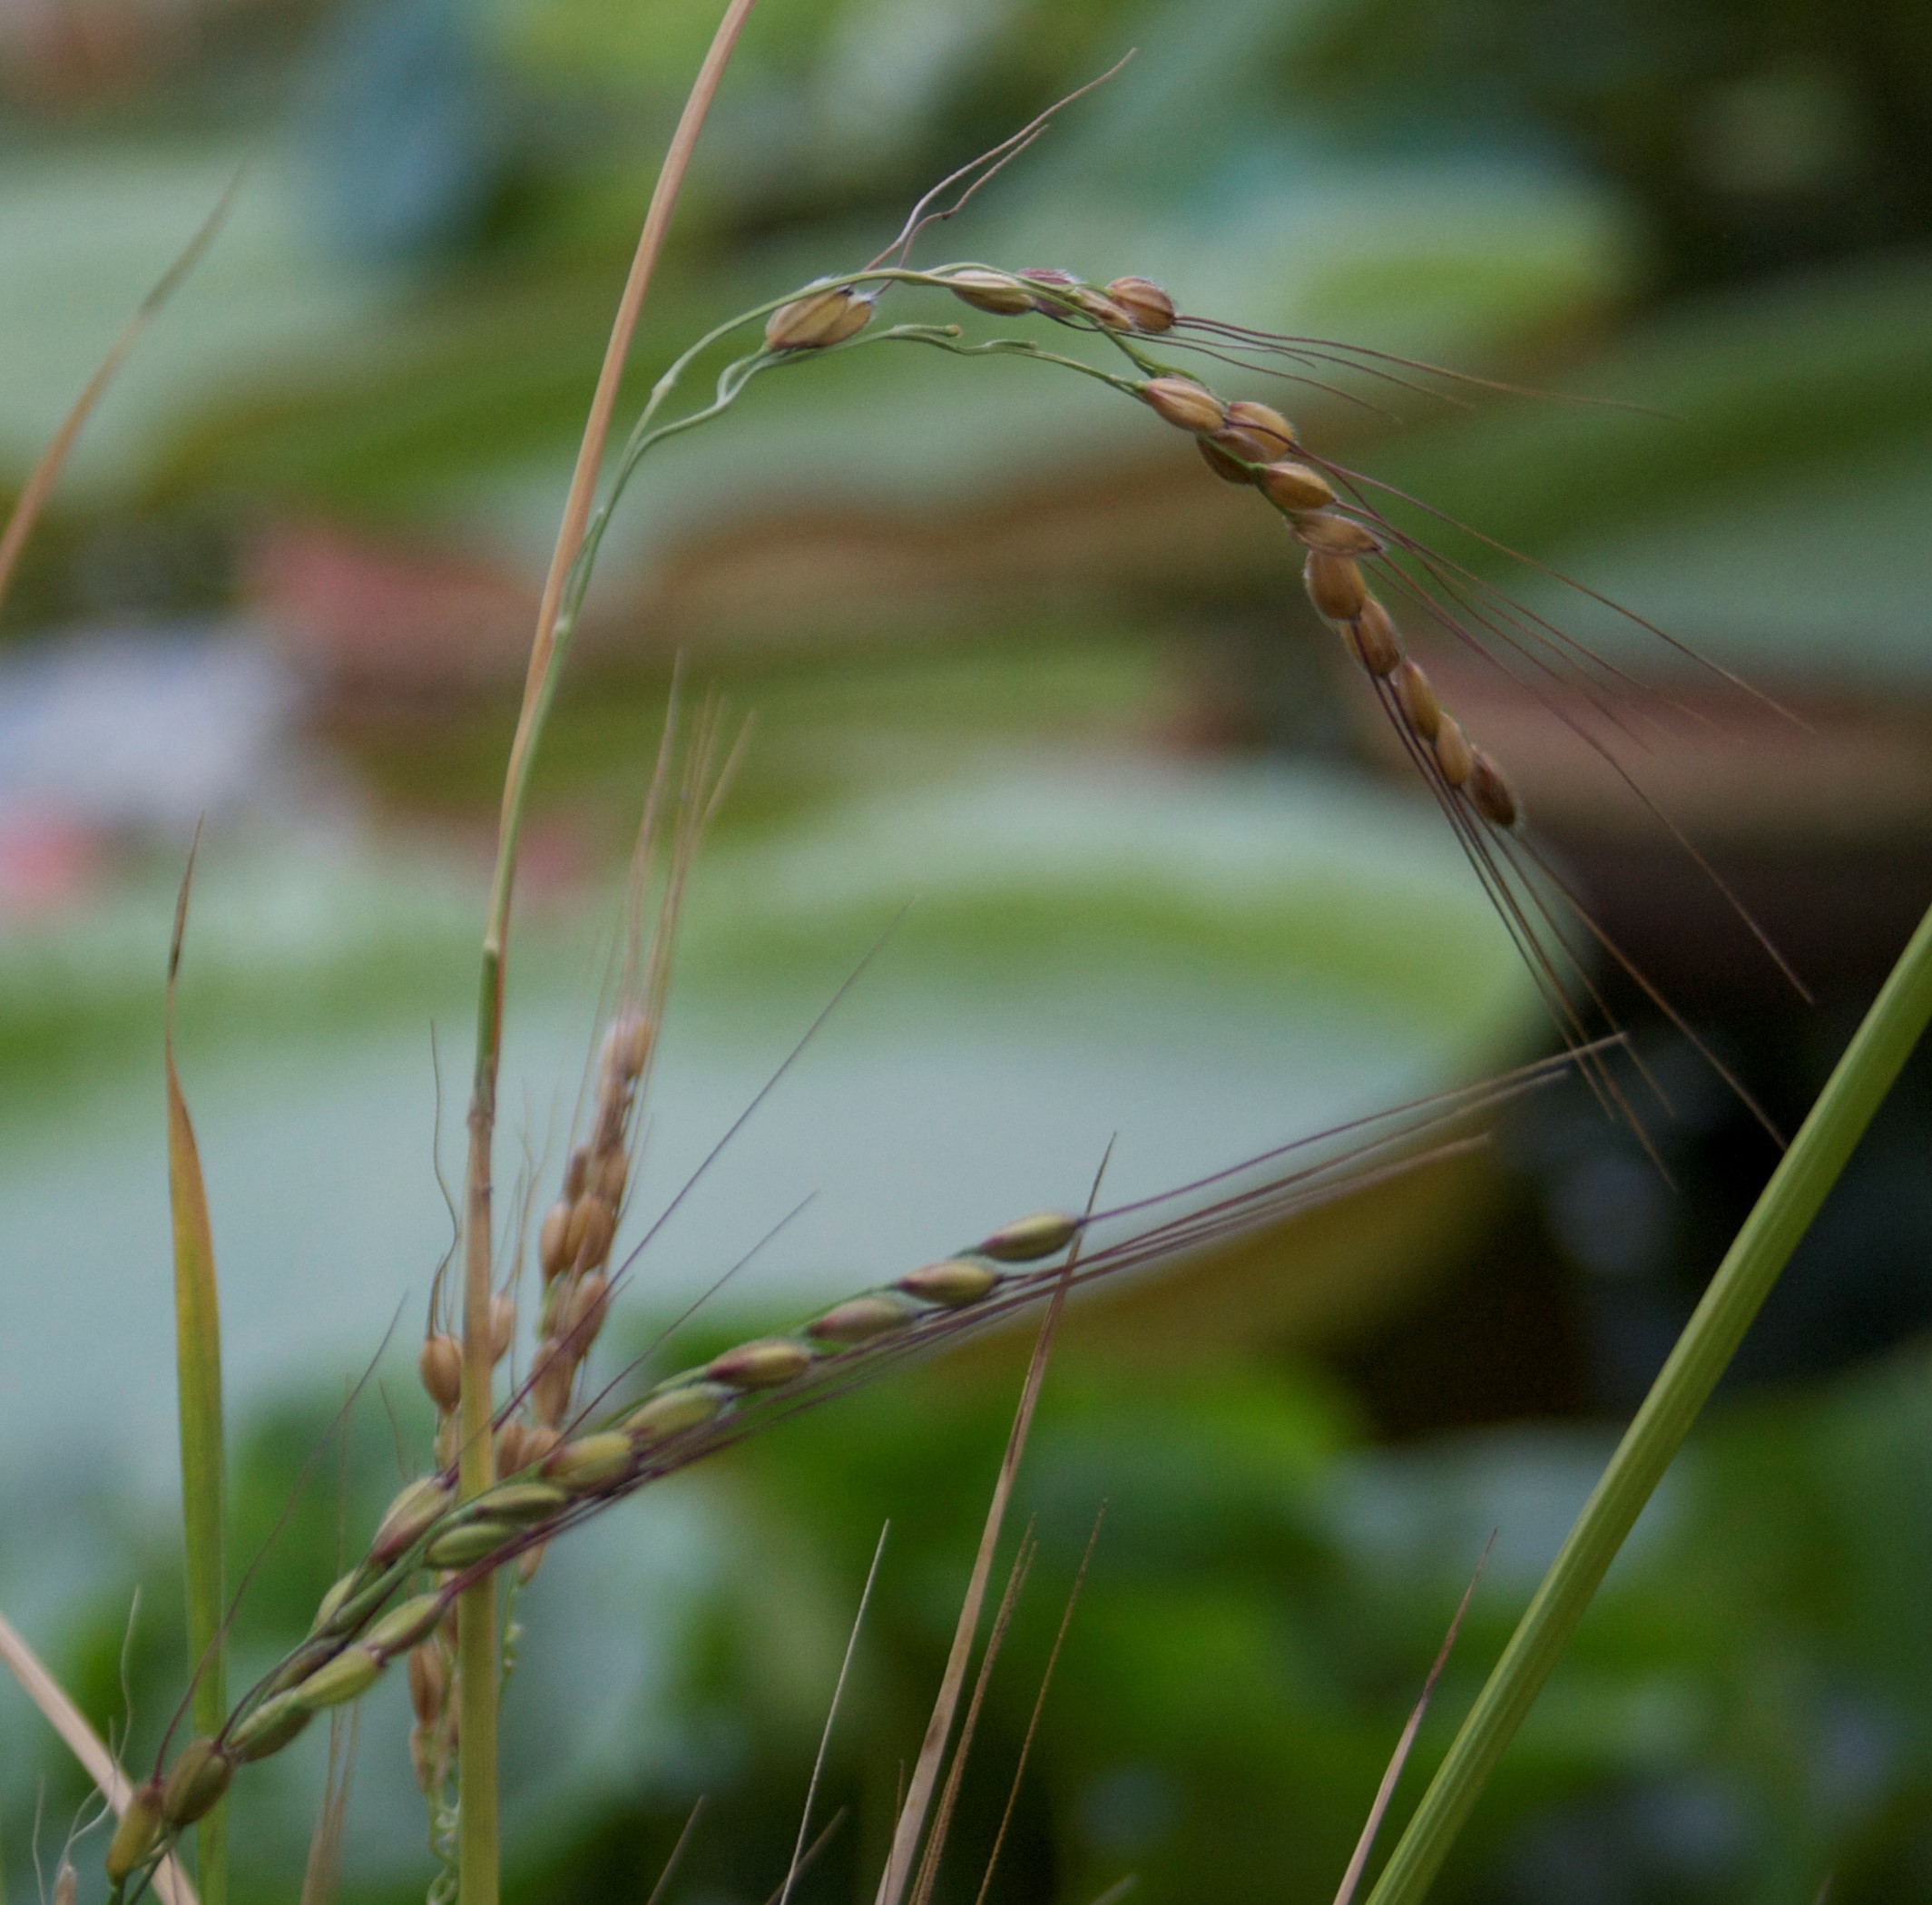
\includegraphics[width=0.5\linewidth]{../images/oryza rufipogon} \caption{\textit{Oryza rufipogon} panicle.}\label{fig:oryza-rufipogon}
\end{figure}

\begin{figure}
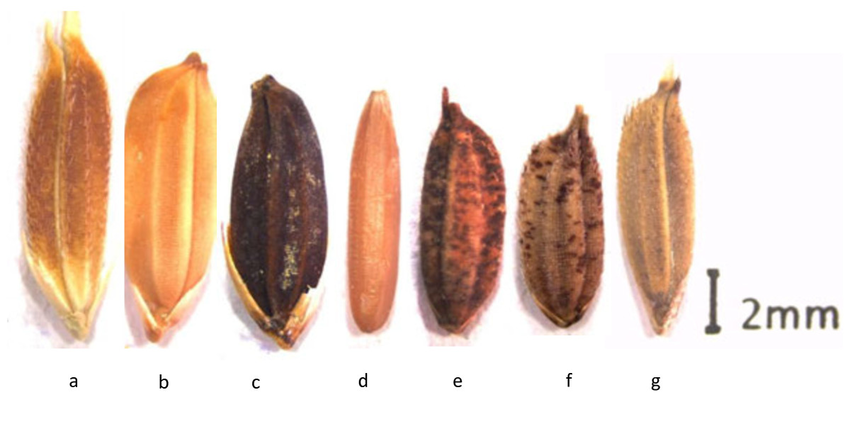
\includegraphics[width=0.6\linewidth]{../images/undehusked_rice_types} \caption{Undehusked seeds of African Oryza species. (a) Oryza longistaminata (b) Oryza glaberrima 1 (c) Oryza glaberrima 2 (d) Oryza brachyantha (e) Oryza eichingeri (f) Oryza punctata (g) Oryza barthii.}\label{fig:oryza-rice-types-seed}
\end{figure}

\ecolumns
\end{frame}

\begin{frame}{Rice phylogeny and history in literatures}
\protect\hypertarget{rice-phylogeny-and-history-in-literatures}{}
\bcolumns
\column{0.4\textwidth}

\begin{itemize}
\tightlist
\item
  Phylogeny of the genus Oryza as revealed by molecular approaches,
  Volume IV, Rice Genetics, 2001.
\item
  Evolution and domestication of Rice, Volume IV, Rice Genetics, 2001.
\end{itemize}

\column{0.6\textwidth}

\begin{figure}
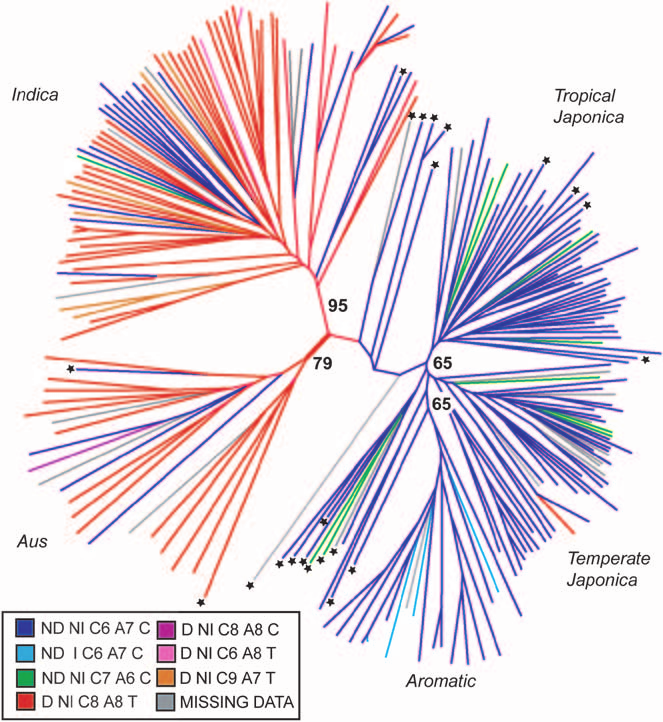
\includegraphics[width=0.6\linewidth]{../images/oryza_genus_phylogenetic_relationship} \caption{Unrooted neighbor-joining tree based on C.S. Chord (1967) based on 169 nuclear SSRs. The key relates the color of the line to the chloroplast haplotype based on ORF100 and PS-ID sequences. Admixed individuals are identified with an asterisk. Bootstrap values (out of 100) are indicated at the branch points. Source: \cite{garris2005genetic}.}\label{fig:oryza-phylogenetic-relationship}
\end{figure}

\ecolumns
\end{frame}

\begin{frame}{}
\protect\hypertarget{section-9}{}
\begin{itemize}
\tightlist
\item
  First archaeological evidence of rice cultivation leads to Yangtze
  valley of eastern China.
\item
  Domestication has resulted in alterations to a large array of
  morphological traits:

  \begin{itemize}
  \tightlist
  \item
    Seed shattering behavior
  \item
    Grain coloration
  \item
    Grain size enlargement
  \item
    Prostrate to erect growth habit
  \item
    Reduced seed dormancy
  \end{itemize}
\item
  Genetic factors contributing to domestication syndrome
  \emph{Shattering4 (Sha4)} on chromosome 4 and black hull by
  \emph{Black hull (Bh4)} on chromosome 4.
\end{itemize}
\end{frame}

\begin{frame}{Maize: History and origin}
\protect\hypertarget{maize-history-and-origin}{}
\begin{itemize}
\tightlist
\item
  Domestication history based on 7100 year old maize pollen from San
  Andres.
\item
  Initially cultivated in seasonal tropical forest of southwestern
  mexico.
\item
  Originated from annual teosinte (\emph{Zea mays} subspecies
  \emph{parviglumis}) around 9000 years ago in mid to lowland regions.
\item
  Later on admixture occured among \emph{parviglumis} and
  \emph{mexicana} (highland type) subspecies.
\end{itemize}
\end{frame}

\begin{frame}{}
\protect\hypertarget{section-10}{}
\bcolumns
\column{0.5\textwidth}

\begin{center}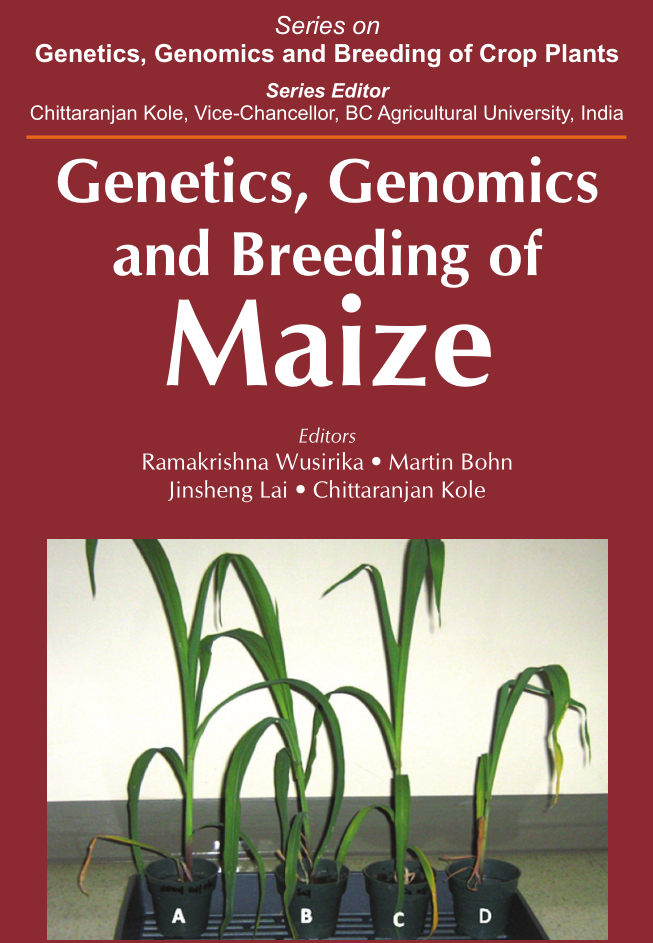
\includegraphics[width=0.75\linewidth]{../images/maize_synthesis_book} \end{center}

\column{0.5\textwidth}

\begin{center}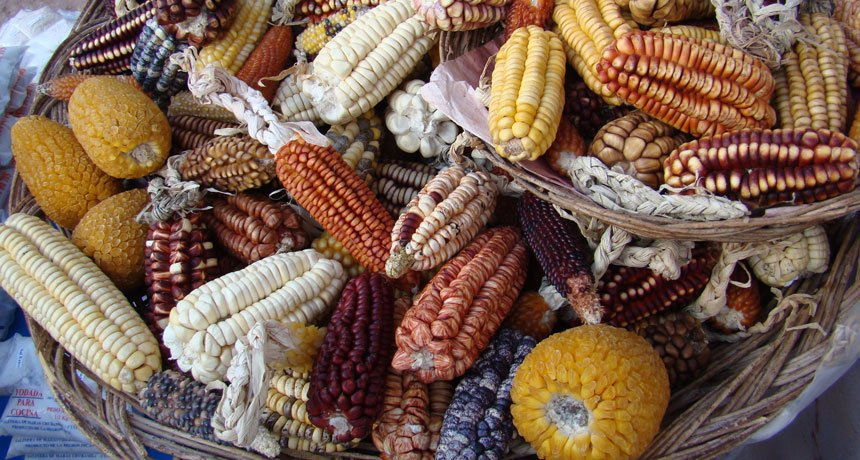
\includegraphics[width=0.99\linewidth]{../images/maize_diversity} \end{center}

\ecolumns
\end{frame}

\begin{frame}{Wheat: History and origin}
\protect\hypertarget{wheat-history-and-origin}{}
\begin{figure}
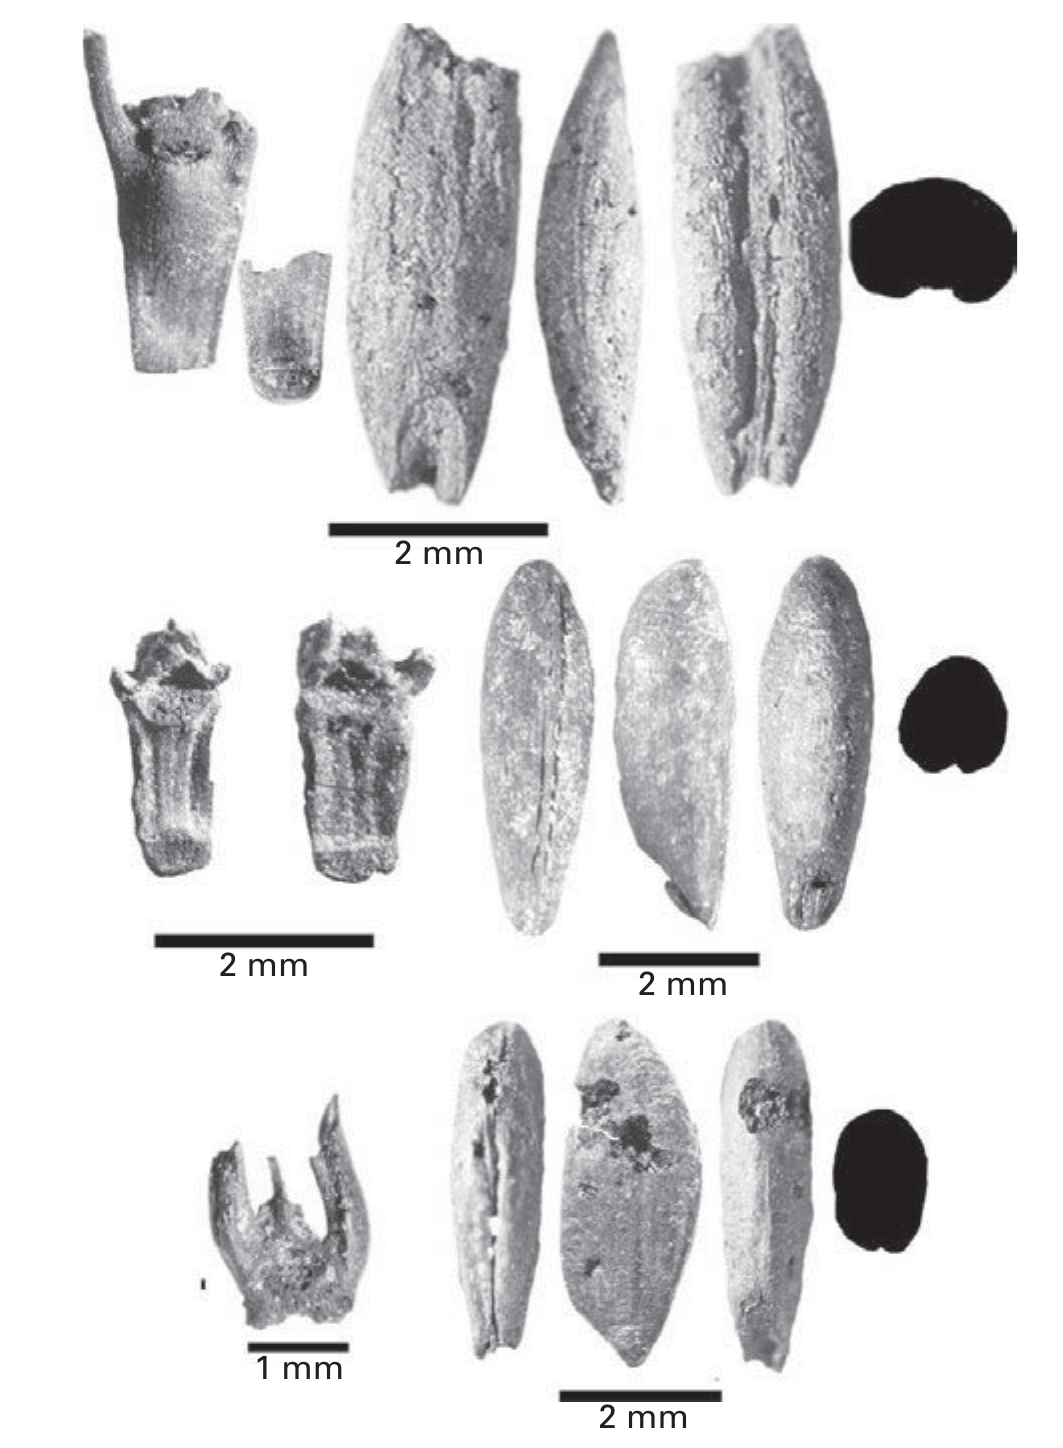
\includegraphics[width=0.3\linewidth]{./../images/charred_grass_grains} \caption{Charred wild cereal spikelet bases (left) and grains (right). Top, Hordeum spontaneum (wild barley) from Jerf el Ahmar. Middle, Secale sp. (rye) from Jerf el Ahmar. Bottom, Triticum boeoticum (single-grain einkorn) from Tell Qaramel. Note the basal abscission scar seen in the barley (top row, second from the left) and for rye the lower end of the rye spikelet bases (second row, first and second from left) is more reliable than the upper scar for distinguishing between wild and domestic.}\label{fig:wheat-barley-archaeology}
\end{figure}
\end{frame}

\hypertarget{megacentres-of-cutivated-plants}{%
\section{Megacentres of cutivated
plants}\label{megacentres-of-cutivated-plants}}

\begin{frame}{}
\protect\hypertarget{section-11}{}
\begin{figure}
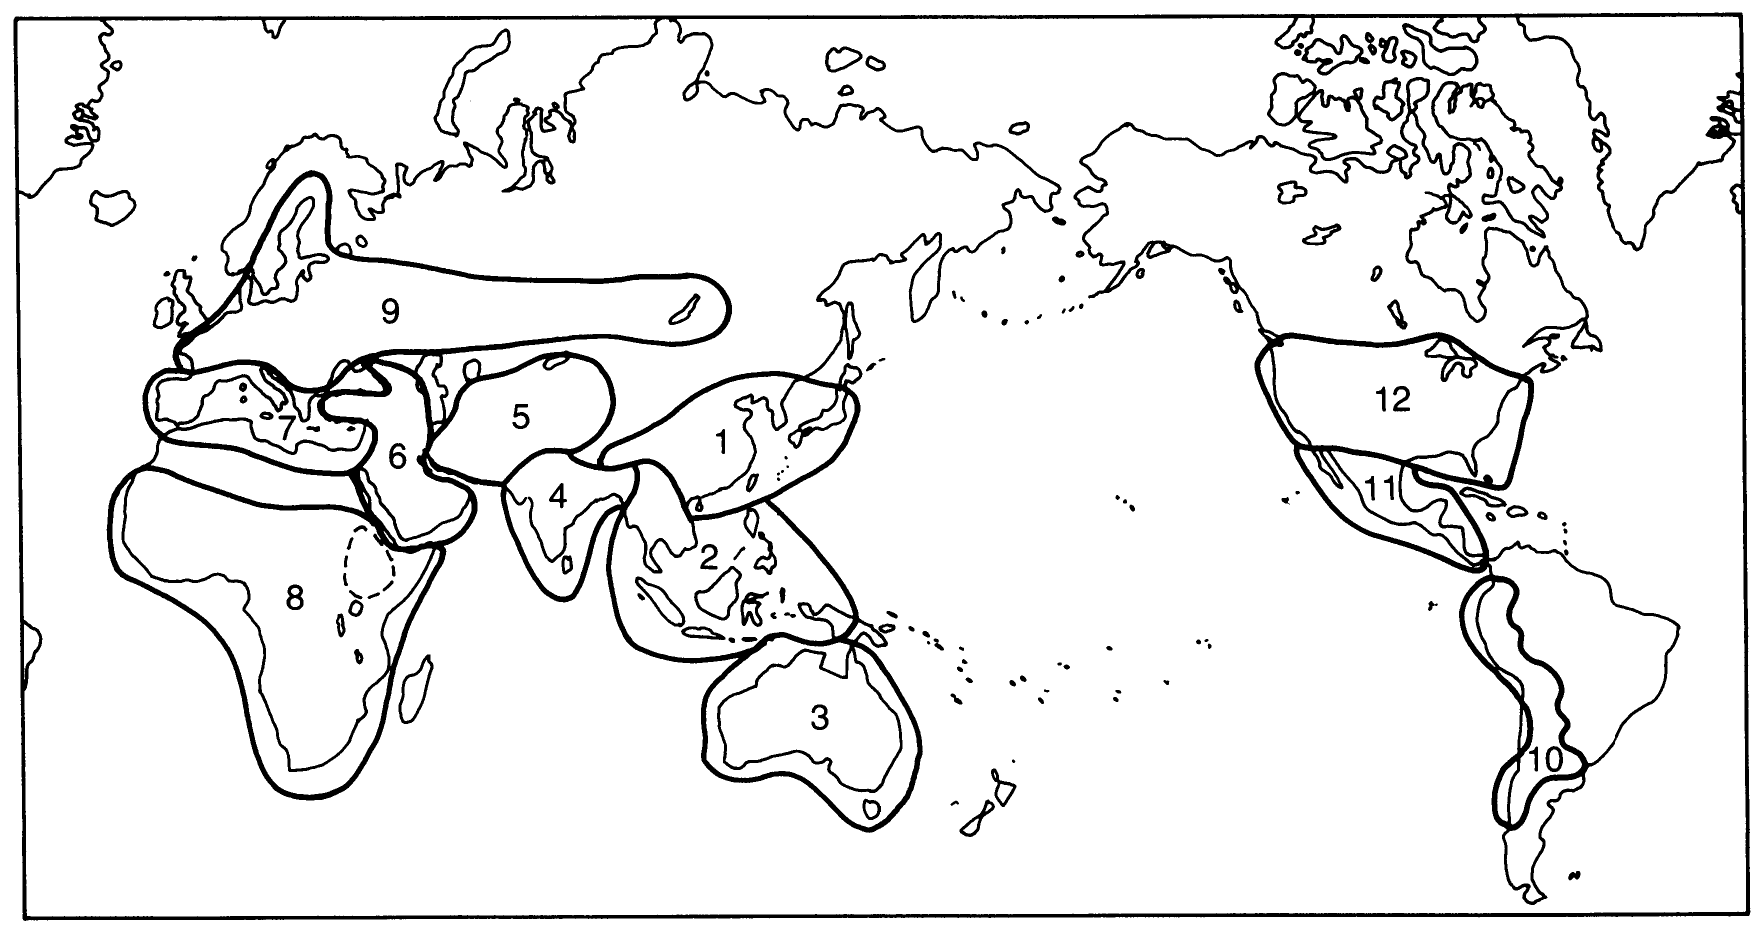
\includegraphics[width=0.55\linewidth]{./../images/megacentres_cultivated} \caption{Megacentres of cultivated plants (Zeven and Zhukovsky, 1975); \cite{hayward2012plant}, Page 37}\label{fig:cultivated-megacentres}
\end{figure}
\end{frame}

\begin{frame}{}
\protect\hypertarget{section-12}{}
\begin{table}

\caption{\label{tab:diversity-region1}Cultivated plants and their regions of diversity. Based on Zeven and Zhukovsky (1975) and Zeven and de Wet (1982); \cite{hayward2012plant}, Page 54, 55.}
\centering
\fontsize{6}{8}\selectfont
\begin{tabular}[t]{>{\raggedright\arraybackslash}p{3em}>{\raggedright\arraybackslash}p{14em}>{\raggedright\arraybackslash}p{32em}}
\toprule
SN & Region & Crops\\
\midrule
\textbf{\cellcolor{gray!6}{1}} & \cellcolor{gray!6}{Chinese-Japanese region} & \cellcolor{gray!6}{Prosomillet, Foxtail millet, Naked oat}\\
\textbf{} &  & Soybean, Adzuki bean\\
\textbf{\cellcolor{gray!6}{}} & \cellcolor{gray!6}{} & \cellcolor{gray!6}{Leafy mustard}\\
\textbf{} &  & Orange/Citrus, Peach, Apricot, Litchi\\
\textbf{\cellcolor{gray!6}{}} & \cellcolor{gray!6}{} & \cellcolor{gray!6}{Bamboo, Ramie, Tung oil tree, Tea}\\
\addlinespace
\textbf{2} & Indochinese-Indonesian region & Rice\\
\textbf{\cellcolor{gray!6}{}} & \cellcolor{gray!6}{} & \cellcolor{gray!6}{Rice bean, Winged bean}\\
\textbf{} &  & Cucurbits/Ash gourd\\
\textbf{\cellcolor{gray!6}{}} & \cellcolor{gray!6}{} & \cellcolor{gray!6}{Mango, Banana, Rambutan, Durian, Bread fruit, Citrus/Lime, Grapefruit}\\
\textbf{} &  & Bamboos, Nutmeg, Clove, Sago-palm, Ginger, Taros and Yams, Betel nut, Coconut\\
\addlinespace
\textbf{\cellcolor{gray!6}{3}} & \cellcolor{gray!6}{Australian region} & \cellcolor{gray!6}{Eucalyptus, Acacia, Macadamia nut}\\
\textbf{4} & Hindustani region & Rice, Little millet\\
\textbf{\cellcolor{gray!6}{}} & \cellcolor{gray!6}{} & \cellcolor{gray!6}{Black gram, Green gram, Moth bean, Rice bean, Dolichos bean, Pigeonpea, Cowpea, Chickpea, Horsegram, Jute}\\
\textbf{} &  & Eggplant, Okra, Cucumber, Leafy mustard, Rat's tail radish, Taros and Yams\\
\textbf{\cellcolor{gray!6}{}} & \cellcolor{gray!6}{} & \cellcolor{gray!6}{Citrus, Banana, Mango, Sunhemp, Tree cotton}\\
\bottomrule
\end{tabular}
\end{table}
\end{frame}

\begin{frame}{}
\protect\hypertarget{section-13}{}
\begin{table}

\caption{\label{tab:diversity-region2}Cultivated plants and their regions of diversity. Based on Zeven and Zhukovsky (1975) and Zeven and de Wet (1982); \cite{hayward2012plant}, Page 54, 55.}
\centering
\fontsize{6}{8}\selectfont
\begin{tabular}[t]{>{\raggedright\arraybackslash}p{3em}>{\raggedright\arraybackslash}p{14em}>{\raggedright\arraybackslash}p{32em}}
\toprule
SN & Region & Crops\\
\midrule
\textbf{\cellcolor{gray!6}{}} & \cellcolor{gray!6}{} & \cellcolor{gray!6}{Sesame, Ginger, Turmeric, Cardamom, Arecanut, Sugarcane, Black pepper, Indigo}\\
\textbf{5} & Central Asian region & Wheat (Bread/Club/Shot), Rye\\
\textbf{\cellcolor{gray!6}{}} & \cellcolor{gray!6}{} & \cellcolor{gray!6}{Allium/Onion, Garlic, Spinach, Peas, Beetroot, Faba bean}\\
\textbf{} &  & Lentil, Chickpea\\
\textbf{\cellcolor{gray!6}{}} & \cellcolor{gray!6}{} & \cellcolor{gray!6}{Apricot, Plum, Pear, Apple, Walnut, Almond, Pistachio, Melon, Grape, Carrot, Radish}\\
\addlinespace
\textbf{} &  & Hemp/Cannabis, Sesame, Flax, Safflower\\
\textbf{\cellcolor{gray!6}{6}} & \cellcolor{gray!6}{Near Eastern region} & \cellcolor{gray!6}{Wheat (Einkorn, Durum, Poulard, Bread), Barley, Rye/Secale}\\
\textbf{} &  & Faba bean, Chickpea, French bean, Lentil, Pea\\
\textbf{\cellcolor{gray!6}{}} & \cellcolor{gray!6}{} & \cellcolor{gray!6}{Brassica oleracea, Allium, Melon, Grape, Plum, Pear, Apple, Apricot, Pistachio, Fig, Pomegranate, Almond}\\
\textbf{} &  & Safflower, Sesame, Flax\\
\addlinespace
\textbf{\cellcolor{gray!6}{}} & \cellcolor{gray!6}{} & \cellcolor{gray!6}{Lupins, Medics}\\
\textbf{7} & Mediterranean region & Wheat (Durum, Turgidum), Oats\\
\textbf{\cellcolor{gray!6}{}} & \cellcolor{gray!6}{} & \cellcolor{gray!6}{Brassica oleracea, Lettuce, Beetroot, Colza}\\
\textbf{} &  & Faba bean, Radish\\
\textbf{\cellcolor{gray!6}{}} & \cellcolor{gray!6}{} & \cellcolor{gray!6}{Olive, Trifolium/Berseem, Lupins, Crocus, Grape, Fennel, Cumin, Celery, Linseed}\\
\bottomrule
\end{tabular}
\end{table}
\end{frame}

\begin{frame}{}
\protect\hypertarget{section-14}{}
\begin{table}

\caption{\label{tab:diversity-region3}Cultivated plants and their regions of diversity. Based on Zeven and Zhukovsky (1975) and Zeven and de Wet (1982); \cite{hayward2012plant}, Page 54, 55.}
\centering
\fontsize{6}{8}\selectfont
\begin{tabular}[t]{>{\raggedright\arraybackslash}p{3em}>{\raggedright\arraybackslash}p{14em}>{\raggedright\arraybackslash}p{32em}}
\toprule
SN & Region & Crops\\
\midrule
\textbf{\cellcolor{gray!6}{8}} & \cellcolor{gray!6}{African region} & \cellcolor{gray!6}{Wheat (Durum, Emmer, Poulard, Bread)}\\
\textbf{} &  & African rice, Sorghum, Pearl millet, Finger millet, Teff\\
\textbf{\cellcolor{gray!6}{}} & \cellcolor{gray!6}{} & \cellcolor{gray!6}{Cowpea, Bottle gourd, Okra, Yams, Cucumber}\\
\textbf{} &  & Castor bean, Sesame, Niger, Oil palm, Safflower, Flax\\
\textbf{\cellcolor{gray!6}{}} & \cellcolor{gray!6}{} & \cellcolor{gray!6}{Cotton, Kenaf, Coffee}\\
\addlinespace
\textbf{} &  & Kola, Bambara, Groundnut, Date palm, Ensete, Melons\\
\textbf{\cellcolor{gray!6}{9}} & \cellcolor{gray!6}{European-siberian region} & \cellcolor{gray!6}{Peach, Pear, Plum, Apricot, Apple, Almond, Walnut, Pistachio, Cherry}\\
\textbf{} &  & Cannabis, Mustard (black), Chicory, Hops, Lettuce\\
\textbf{\cellcolor{gray!6}{10}} & \cellcolor{gray!6}{South American region} & \cellcolor{gray!6}{Potato, Sweet potato, Xanthosoma}\\
\textbf{} &  & Lima bean, Amaranth, Chenopodium, Cucurbita, Tomato, Tobacco, Lupin\\
\addlinespace
\textbf{\cellcolor{gray!6}{}} & \cellcolor{gray!6}{} & \cellcolor{gray!6}{Papaya, Pineapple}\\
\textbf{} &  & Groundnut, Sea island cotton\\
\textbf{\cellcolor{gray!6}{}} & \cellcolor{gray!6}{} & \cellcolor{gray!6}{Cassava, Cacao, Rubber tree, Passion fruit}\\
\textbf{11} & Central American and Mexican region & Maize, French bean, Potato, Cucurbita, Pepper/Chilli, Amaranth, Chenopodium, Tobacco, Sisal hemp, Upland cotton\\
\textbf{\cellcolor{gray!6}{12}} & \cellcolor{gray!6}{North American region} & \cellcolor{gray!6}{Jeruselum artichoke, Sunflower, Plum, Raspberry, Strawberry}\\
\bottomrule
\end{tabular}
\end{table}
\end{frame}

\renewcommand\refname{Bibliography}
\begin{frame}[allowframebreaks]{Bibliography}
  \bibliographytrue
  \bibliography{../bibliography/bibliographies.bib}
\end{frame}

\end{document}
